\section{Analysis}

\subsection{Limitations}
Whether \textsc{Network Diversion} in the general case can be solved in polynomial time is still an open problem.
This algorithm does not solve the general case, but rather the special case where the input graph...
\begin{itemize}
    \item is planar,
    \item is undirected,
    \item has edges of either non-negative weights or no weights at all.
\end{itemize}

% In addition, even though the algorithm as described here will also work on non-simple graphs, we implemented the algorithm with the assumption that the graph is simple. See \Cref{chapter:codebase} for more details. \todo{vurder å skrive dette i kodekapitlet istedet. Eller også ta med at vi trenger en straight-line embedding.}

\subsection{Complexity}
\label{subsection:network-diversion-complexity}
Let $(G, s, t, d)$ be an instance of \textsc{Network Diversion}, and let $n := |V|$. \\
Claim: our algorithm runs in time $O(n \log n)$.

\begin{proof}
    We find first a shortest $s$-$t$-path in $G$ that does not use $d$, in time $O(n+m)$.

    Then we subdivide all the edges in $G^\star$ except those found in the path, in time $O(n+m)$. This new graph has size $n' \leq 2n \in O(n)$ and $m' \leq 2m \in O(m)$.

    Next up is to find an odd path in the subdivided graph, in time $O(m' \log n') = O(m \log n)$.

    Lastly, if we are interested in the specific set of edges in the diversion and not just the cost, we un-subdivide the odd path in time $O(n') = O(n)$.

    In total, we have a running time of $O(n+m) + O(m \log n) + O(n) = O(m \log n)$. Since $G$ is planar we have that $m \in O(n)$, and we can simplify the complexity to just $O(n \log n)$, which completes the proof.
\end{proof}

Note that here we have assumed that the dual graph $G^\star$ has already been computed prior to starting the algorithm. If we have a straight-line embedding of $G$ we can compute $G^\star$ in $O(n+m)$, which would not change the overall running time. However, if we do not have such an embedding the total running time might be considerably more.

\subsection{Benchmarking}
We compare the theoretical and practical running times on Delaunay graphs, like we did in \Cref{subsubsection:odd-path-delaunay-testing}. For each graph, we have estimated a source and target vertex of maximum distance between each other, and picked three edges in the graph as diversion edges. We pick whichever diversion edge leads to the worst running time over 20 attempts, and plot the median over those 20 attempts.

Here too have we tried to create a function out of the theoretical running time of $O(n \log n)$, this time with different constants. We have set $m := 3n$ in the plot.

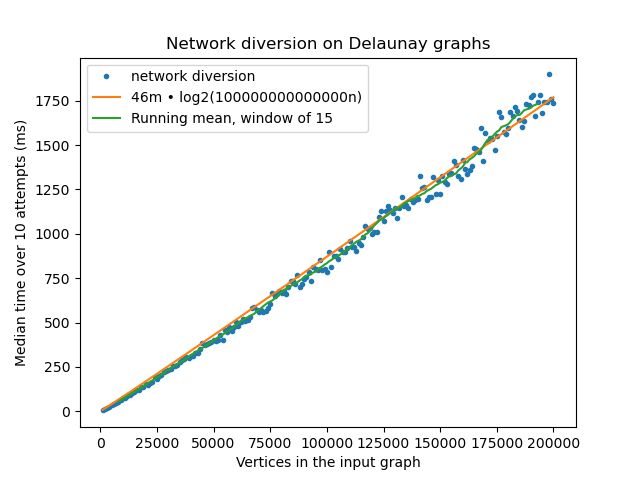
\includegraphics[width=12cm]{figures/bench_plots/network diversion.png}

As we can see, the running times grow just barely more than linearly compared to the input size. This is not surprising considering the linearithmic theoretical running time.

\todo[inline]{Benchmarking on real graphs}

\todo[inline]{Visualize the diversion set}

\subsection{Discussion}
\todo[inline]{Write some kickass discussion here}